% !TEX encoding = UTF-8 Unicode
%% bare_conf_compsoc.tex
%% V1.4b
%% 2015/08/26
%% by Michael Shell
%% See:
%% http://www.michaelshell.org/
%% for current contact information.
%%
%% This is a skeleton file demonstrating the use of IEEEtran.cls
%% (requires IEEEtran.cls version 1.8b or later) with an IEEE Computer
%% Society conference paper.
%%
%% Support sites:
%% http://www.michaelshell.org/tex/ieeetran/
%% http://www.ctan.org/pkg/ieeetran
%% and
%% http://www.ieee.org/

%%*************************************************************************
%% Legal Notice:
%% This code is offered as-is without any warranty either expressed or
%% implied; without even the implied warranty of MERCHANTABILITY or
%% FITNESS FOR A PARTICULAR PURPOSE! 
%% User assumes all risk.
%% In no event shall the IEEE or any contributor to this code be liable for
%% any damages or losses, including, but not limited to, incidental,
%% consequential, or any other damages, resulting from the use or misuse
%% of any information contained here.
%%
%% All comments are the opinions of their respective authors and are not
%% necessarily endorsed by the IEEE.
%%
%% This work is distributed under the LaTeX Project Public License (LPPL)
%% ( http://www.latex-project.org/ ) version 1.3, and may be freely used,t
%% distributed and modified. A copy of the LPPL, version 1.3, is included
%% in the base LaTeX documentation of all distributions of LaTeX released
%% 2003/12/01 or later.
%% Retain all contribution notices and credits.
%% ** Modified files should be clearly indicated as such, including  **
%% ** renaming them and changing author support contact information. **
%%*************************************************************************


% *** Authors should verify (and, if needed, correct) their LaTeX system  ***
% *** with the testflow diagnostic prior to trusting their LaTeX platform ***
% *** with production work. The IEEE's font choices and paper sizes can   ***
% *** trigger bugs that do not appear when using other class files.       ***                          ***
% The testflow support page is at:
% http://www.michaelshell.org/tex/testflow/



\documentclass[conference,compsoc]{IEEEtran}
% Some/most Computer Society conferences require the compsoc mode option,
% but others may want the standard conference format.
%
% If IEEEtran.cls has not been installed into the LaTeX system files,
% manually specify the path to it like:
% \documentclass[conference,compsoc]{../sty/IEEEtran}





% Some very useful LaTeX packages include:
% (uncomment the ones you want to load)


% *** MISC UTILITY PACKAGES ***
%
%\usepackage{ifpdf}
% Heiko Oberdiek's ifpdf.sty is very useful if you need conditional
% compilation based on whether the output is pdf or dvi.
% usage:
% \ifpdf
%   % pdf code
% \else
%   % dvi code
% \fi
% The latest version of ifpdf.sty can be obtained from:
% http://www.ctan.org/pkg/ifpdf
% Also, note that IEEEtran.cls V1.7 and later provides a builtin
% \ifCLASSINFOpdf conditional that works the same way.
% When switching from latex to pdflatex and vice-versa, the compiler may
% have to be run twice to clear warning/error messages.


\usepackage[utf8]{inputenc}
\usepackage[portuguese]{babel}

\usepackage{url}
\usepackage{hyperref} 
\usepackage{graphicx}
\usepackage{fancyref}
\usepackage{amsmath}
\usepackage{fancyhdr}
\pagestyle{fancy}

% *** CITATION PACKAGES ***
%
\ifCLASSOPTIONcompsoc
  % IEEE Computer Society needs nocompress option
  % requires cite.sty v4.0 or later (November 2003)
  \usepackage[nocompress]{cite}
\else
  % normal IEEE
  \usepackage{cite}
\fi
% cite.sty was written by Donald Arseneau
% V1.6 and later of IEEEtran pre-defines the format of the cite.sty package
% \cite{} output to follow that of the IEEE. Loading the cite package will
% result in citation numbers being automatically sorted and properly
% "compressed/ranged". e.g., [1], [9], [2], [7], [5], [6] without using
% cite.sty will become [1], [2], [5]--[7], [9] using cite.sty. cite.sty's
% \cite will automatically add leading space, if needed. Use cite.sty's
% noadjust option (cite.sty V3.8 and later) if you want to turn this off
% such as if a citation ever needs to be enclosed in parenthesis.
% cite.sty is already installed on most LaTeX systems. Be sure and use
% version 5.0 (2009-03-20) and later if using hyperref.sty.
% The latest version can be obtained at:
% http://www.ctan.org/pkg/cite
% The documentation is contained in the cite.sty file itself.
%
% Note that some packages require special options to format as the Computer
% Society requires. In particular, Computer Society  papers do not use
% compressed citation ranges as is done in typical IEEE papers
% (e.g., [1]-[4]). Instead, they list every citation separately in order
% (e.g., [1], [2], [3], [4]). To get the latter we need to load the cite
% package with the nocompress option which is supported by cite.sty v4.0
% and later.





% *** GRAPHICS RELATED PACKAGES ***
%
\ifCLASSINFOpdf
  % \usepackage[pdftex]{graphicx}
  % declare the path(s) where your graphic files are
  % \graphicspath{{../pdf/}{../jpeg/}}
  % and their extensions so you won't have to specify these with
  % every instance of \includegraphics
  % \DeclareGraphicsExtensions{.pdf,.jpeg,.png}
\else
  % or other class option (dvipsone, dvipdf, if not using dvips). graphicx
  % will default to the driver specified in the system graphics.cfg if no
  % driver is specified.
  % \usepackage[dvips]{graphicx}
  % declare the path(s) where your graphic files are
  % \graphicspath{{../eps/}}
  % and their extensions so you won't have to specify these with
  % every instance of \includegraphics
  % \DeclareGraphicsExtensions{.eps}
\fi
% graphicx was written by David Carlisle and Sebastian Rahtz. It is
% required if you want graphics, photos, etc. graphicx.sty is already
% installed on most LaTeX systems. The latest version and documentation
% can be obtained at: 
% http://www.ctan.org/pkg/graphicx
% Another good source of documentation is "Using Imported Graphics in
% LaTeX2e" by Keith Reckdahl which can be found at:
% http://www.ctan.org/pkg/epslatex
%
% latex, and pdflatex in dvi mode, support graphics in encapsulated
% postscript (.eps) format. pdflatex in pdf mode supports graphics
% in .pdf, .jpeg, .png and .mps (metapost) formats. Users should ensure
% that all non-photo figures use a vector format (.eps, .pdf, .mps) and
% not a bitmapped formats (.jpeg, .png). The IEEE frowns on bitmapped formats
% which can result in "jaggedy"/blurry rendering of lines and letters as
% well as large increases in file sizes.
%
% You can find documentation about the pdfTeX application at:
% http://www.tug.org/applications/pdftex





% *** MATH PACKAGES ***
%
%\usepackage{amsmath}
% A popular package from the American Mathematical Society that provides
% many useful and powerful commands for dealing with mathematics.
%
% Note that the amsmath package sets \interdisplaylinepenalty to 10000
% thus preventing page breaks from occurring within multiline equations. Use:
%\interdisplaylinepenalty=2500
% after loading amsmath to restore such page breaks as IEEEtran.cls normally
% does. amsmath.sty is already installed on most LaTeX systems. The latest
% version and documentation can be obtained at:
% http://www.ctan.org/pkg/amsmath





% *** SPECIALIZED LIST PACKAGES ***
%
%\usepackage{algorithmic}
% algorithmic.sty was written by Peter Williams and Rogerio Brito.
% This package provides an algorithmic environment fo describing algorithms.
% You can use the algorithmic environment in-text or within a figure
% environment to provide for a floating algorithm. Do NOT use the algorithm
% floating environment provided by algorithm.sty (by the same authors) or
% algorithm2e.sty (by Christophe Fiorio) as the IEEE does not use dedicated
% algorithm float types and packages that provide these will not provide
% correct IEEE style captions. The latest version and documentation of
% algorithmic.sty can be obtained at:
% http://www.ctan.org/pkg/algorithms
% Also of interest may be the (relatively newer and more customizable)
% algorithmicx.sty package by Szasz Janos:
% http://www.ctan.org/pkg/algorithmicx




% *** ALIGNMENT PACKAGES ***
%
%\usepackage{array}
% Frank Mittelbach's and David Carlisle's array.sty patches and improves
% the standard LaTeX2e array and tabular environments to provide better
% appearance and additional user controls. As the default LaTeX2e table
% generation code is lacking to the point of almost being broken with
% respect to the quality of the end results, all users are strongly
% advised to use an enhanced (at the very least that provided by array.sty)
% set of table tools. array.sty is already installed on most systems. The
% latest version and documentation can be obtained at:
% http://www.ctan.org/pkg/array


% IEEEtran contains the IEEEeqnarray family of commands that can be used to
% generate multiline equations as well as matrices, tables, etc., of high
% quality.




% *** SUBFIGURE PACKAGES ***
%\ifCLASSOPTIONcompsoc
%  \usepackage[caption=false,font=footnotesize,labelfont=sf,textfont=sf]{subfig}
%\else
%  \usepackage[caption=false,font=footnotesize]{subfig}
%\fi
% subfig.sty, written by Steven Douglas Cochran, is the modern replacement
% for subfigure.sty, the latter of which is no longer maintained and is
% incompatible with some LaTeX packages including fixltx2e. However,
% subfig.sty requires and automatically loads Axel Sommerfeldt's caption.sty
% which will override IEEEtran.cls' handling of captions and this will result
% in non-IEEE style figure/table captions. To prevent this problem, be sure
% and invoke subfig.sty's "caption=false" package option (available since
% subfig.sty version 1.3, 2005/06/28) as this is will preserve IEEEtran.cls
% handling of captions.
% Note that the Computer Society format requires a sans serif font rather
% than the serif font used in traditional IEEE formatting and thus the need
% to invoke different subfig.sty package options depending on whether
% compsoc mode has been enabled.
%
% The latest version and documentation of subfig.sty can be obtained at:
% http://www.ctan.org/pkg/subfig




% *** FLOAT PACKAGES ***
%
%\usepackage{fixltx2e}
% fixltx2e, the successor to the earlier fix2col.sty, was written by
% Frank Mittelbach and David Carlisle. This package corrects a few problems
% in the LaTeX2e kernel, the most notable of which is that in current
% LaTeX2e releases, the ordering of single and double column floats is not
% guaranteed to be preserved. Thus, an unpatched LaTeX2e can allow a
% single column figure to be placed prior to an earlier double column
% figure.
% Be aware that LaTeX2e kernels dated 2015 and later have fixltx2e.sty's
% corrections already built into the system in which case a warning will
% be issued if an attempt is made to load fixltx2e.sty as it is no longer
% needed.
% The latest version and documentation can be found at:
% http://www.ctan.org/pkg/fixltx2e


%\usepackage{stfloats}
% stfloats.sty was written by Sigitas Tolusis. This package gives LaTeX2e
% the ability to do double column floats at the bottom of the page as well
% as the top. (e.g., "\begin{figure*}[!b]" is not normally possible in
% LaTeX2e). It also provides a command:
%\fnbelowfloat
% to enable the placement of footnotes below bottom floats (the standard
% LaTeX2e kernel puts them above bottom floats). This is an invasive package
% which rewrites many portions of the LaTeX2e float routines. It may not work
% with other packages that modify the LaTeX2e float routines. The latest
% version and documentation can be obtained at:
% http://www.ctan.org/pkg/stfloats
% Do not use the stfloats baselinefloat ability as the IEEE does not allow
% \baselineskip to stretch. Authors submitting work to the IEEE should note
% that the IEEE rarely uses double column equations and that authors should try
% to avoid such use. Do not be tempted to use the cuted.sty or midfloat.sty
% packages (also by Sigitas Tolusis) as the IEEE does not format its papers in
% such ways.
% Do not attempt to use stfloats with fixltx2e as they are incompatible.
% Instead, use Morten Hogholm'a dblfloatfix which combines the features
% of both fixltx2e and stfloats:
%
% \usepackage{dblfloatfix}
% The latest version can be found at:
% http://www.ctan.org/pkg/dblfloatfix




% *** PDF, URL AND HYPERLINK PACKAGES ***
%
%\usepackage{url}
% url.sty was written by Donald Arseneau. It provides better support for
% handling and breaking URLs. url.sty is already installed on most LaTeX
% systems. The latest version and documentation can be obtained at:
% http://www.ctan.org/pkg/url
% Basically, \url{my_url_here}.




% *** Do not adjust lengths that control margins, column widths, etc. ***
% *** Do not use packages that alter fonts (such as pslatex).         ***
% There should be no need to do such things with IEEEtran.cls V1.6 and later.
% (Unless specifically asked to do so by the journal or conference you plan
% to submit to, of course. )


% correct bad hyphenation here
\hyphenation{op-tical net-works semi-conduc-tor}


\begin{document}
%
% paper title
% Titles are generally capitalized except for words such as a, an, and, as,
% at, but, by, for, in, nor, of, on, or, the, to and up, which are usually
% not capitalized unless they are the first or last word of the title.
% Linebreaks \\ can be used within to get better formatting as desired.
% Do not put math or special symbols in the title.
\title{Memória Partilhada: Programação com PThreads}


% author names and affiliations
% use a multiple column layout for up to three different
% affiliations
\author{\IEEEauthorblockN{Sérgio Caldas}
\IEEEauthorblockA{Universidade do Minho\\Escola de Engenharia\\Departamento de Informática\\
Email: a57779@alunos.uminho.pt}}

% conference papers do not typically use \thanks and this command
% is locked out in conference mode. If really needed, such as for
% the acknowledgment of grants, issue a \IEEEoverridecommandlockouts
% after \documentclass

% for over three affiliations, or if they all won't fit within the width
% of the page (and note that there is less available width in this regard for
% compsoc conferences compared to traditional conferences), use this
% alternative format:
% 
%\author{\IEEEauthorblockN{Michael Shell\IEEEauthorrefmark{1},
%Homer Simpson\IEEEauthorrefmark{2},
%James Kirk\IEEEauthorrefmark{3}, 
%Montgomery Scott\IEEEauthorrefmark{3} and
%Eldon Tyrell\IEEEauthorrefmark{4}}
%\IEEEauthorblockA{\IEEEauthorrefmark{1}School of Electrical and Computer Engineering\\
%Georgia Institute of Technology,
%Atlanta, Georgia 30332--0250\\ Email: see http://www.michaelshell.org/contact.html}
%\IEEEauthorblockA{\IEEEauthorrefmark{2}Twentieth Century Fox, Springfield, USA\\
%Email: homer@thesimpsons.com}
%\IEEEauthorblockA{\IEEEauthorrefmark{3}Starfleet Academy, San Francisco, California 96678-2391\\
%Telephone: (800) 555--1212, Fax: (888) 555--1212}
%\IEEEauthorblockA{\IEEEauthorrefmark{4}Tyrell Inc., 123 Replicant Street, Los Angeles, California 90210--4321}}




% use for special paper notices
%\IEEEspecialpapernotice{(Invited Paper)}




% make the title area
\maketitle

\tableofcontents
\vspace{0.5cm}

% As a general rule, do not put math, special symbols or citations
% in the abstract
\begin{abstract}
Este trabalho baseia-se essencialmente na programação em memória partilhada, recorrendo a \textit{POSIX Threads}, mais conhecidas como \textit{PThreads}, estas são muito populares no ambiente \textit{UNIX}. O trabalho divide-se em duas partes, na primeira parte medi o tempo médio de criação de uma \textit{Thread} e a segunda parte desenvolvi um algoritmo (\textit{Trapezoidal Rule}) com recurso a \textit{PThreads}. 
\end{abstract}

% no keywords




% For peer review papers, you can put extra information on the cover
% page as needed:
% \ifCLASSOPTIONpeerreview
% \begin{center} \bfseries EDICS Category: 3-BBND \end{center}
% \fi
%
% For peerreview papers, this IEEEtran command inserts a page break and
% creates the second title. It will be ignored for other modes.
\IEEEpeerreviewmaketitle



\section{Introdução}
Este trabalho, desenvolvido no âmbito da disciplina de Engenharia Sistemas de Computação (ESC), inserida no perfil de Computação Paralela e Distribuída (CPD) do curso de MIEI\footnote{Mestrado Integrado em Engenharia Informática}, consiste no desenvolvimento de programas com recurso a \textit{PThreads}. Este trabalho é dividido em duas partes, na primeira parte desenvolvi um pequeno programa (tipo \textit{Hello World}) em que me media o tempo médio da criação de um fio de execução (\textit{Thread}). Na segunda parte desenvolvi o algoritmo da regra trapezoidal, com recurso a \textit{PThreads}, em que media o tempo de execução para um dado intervalo, no algoritmo existe uma variável que irá ser partilhada por todas as \textit{Threads} e para evitar \textit{Data Races} implementei as técnicas que estudamos para forçar a exclusão mutua, mais precisamente \textit{Busy Waiting, Mutex} e Semáforos.

Neste relatorio encontra-se a análise dos resultados obtidos, tanto para a primeira parte do trabalho, como para a segunda.

\section{Ambiente de testes}
Depois de desenvolvidos os dois algoritmos (relativos a primeira e segunda parte) efetuei testes na minha máquina pessoal e no \textit{Search}, mais precisamente numa máquina 431. A metodologia de testes por mim escolhida foi a de \textit{k-best solution}, esta metodologia baseia-se essencialmente na execução do \textit{Kernel} de \textit{k} vezes escolhendo a melhor solução dessas \textit{k} vezes. O \textit{k} por mim escolhido foi de 5. De referir que foram feitos testes para 1, 2, 4, 8, 16, 32 e 64 \textit{Threads}, sendo que para cada um destes números de \textit{Threads} o \textit{Kernel} foi executado 5 vezes (\textit{k-best solution}).

Na tabela \ref{t:my_laptop} e na tabela \ref{t:431}, encontra-se a caracterização das duas máquinas de teste, isto é, a caracterização da minha máquina e da máquina 431 do \textit{Search}, respetivamente.

\begin{table}[]
\centering
\begin{tabular}{ | l | c | }
\hline
System & MacBook Pro (15-inch, Mid 2010)\\ 
\hline 
\hline
\# CPUs & 1\\ 
\hline
CPU & Intel\textsuperscript{\textregistered} Core\textsuperscript{\texttrademark} I5-520M \\
\hline 
Architecture & Arrandale\\ 
\hline 
\# Cores per CPU & 2\\ 
\hline 
\# Threads per CPU & 4\\ 
\hline 
Clock Freq. & 2.53 GHz\\ 
\hline 
\hline 
L1 Cache & 64 KB \newline 32 KB por core\\ 
\hline 
L2 Cache & 512 KB \newline 256 KB por core\\ 
\hline 
L3 Cache & 3 MB\\ 
\hline 
\hline 
Inst. Set Ext. & SSE4.1/4.2\\
 \hline 
\#Memory Channels & 2\\ 
\hline 
Memory BW & 17.1 GB/s\\
\hline
\end{tabular}
\caption{Caracterização da Máquina Pessoal}
\label{t:my_laptop}
\end{table}


\begin{table}[]
\centering
\begin{tabular}{ | l | c | }
\hline
System & Máquina 431\\ 
\hline 
\hline
\# CPUs & 2\\ 
\hline
CPU & Intel\textsuperscript{\textregistered} Xeon\textsuperscript{\textregistered} X5650\\
\hline 
Architecture & Nehalem\\ 
\hline 
\# Cores per CPU & 6\\ 
\hline 
\# Threads per CPU & 12\\ 
\hline 
Clock Freq. & 2.66 GHz\\ 
\hline 
\hline 
L1 Cache & 192 KB \newline 32 KB por core\\ 
\hline 
L2 Cache & 1536 KB \newline 256 KB por core\\ 
\hline 
L3 Cache & 12 MB\\ 
\hline 
\hline 
Inst. Set Ext. & SSE4.2 e AVX\\
 \hline 
\#Memory Channels & 3\\ 
\hline 
Memory BW & 32 GB/s\\
\hline
\end{tabular}
\caption{Caracterização da Máquina 431}
\label{t:431}
\end{table}


\section{1ª Parte - Tempo Médio de Criação de um Fio de Execução}
Nesta primeira parte do trabalho, desenvolvi um pequeno algoritmo que cria um determinado número de \textit{Threads}, executa uma função (que não faz nada) por cada \textit{Thread}, depois faz \textit{join} a todas as \textit{Threads} e termina o programa. O objetivo deste algoritmo é calcular o tempo médio de criação de um fio de execução (\textit{Thread}), de forma a poder comparar o comportamento do tempo, quando se aumenta o número de \textit{Threads}.

\begin{figure}[h!]
\centering
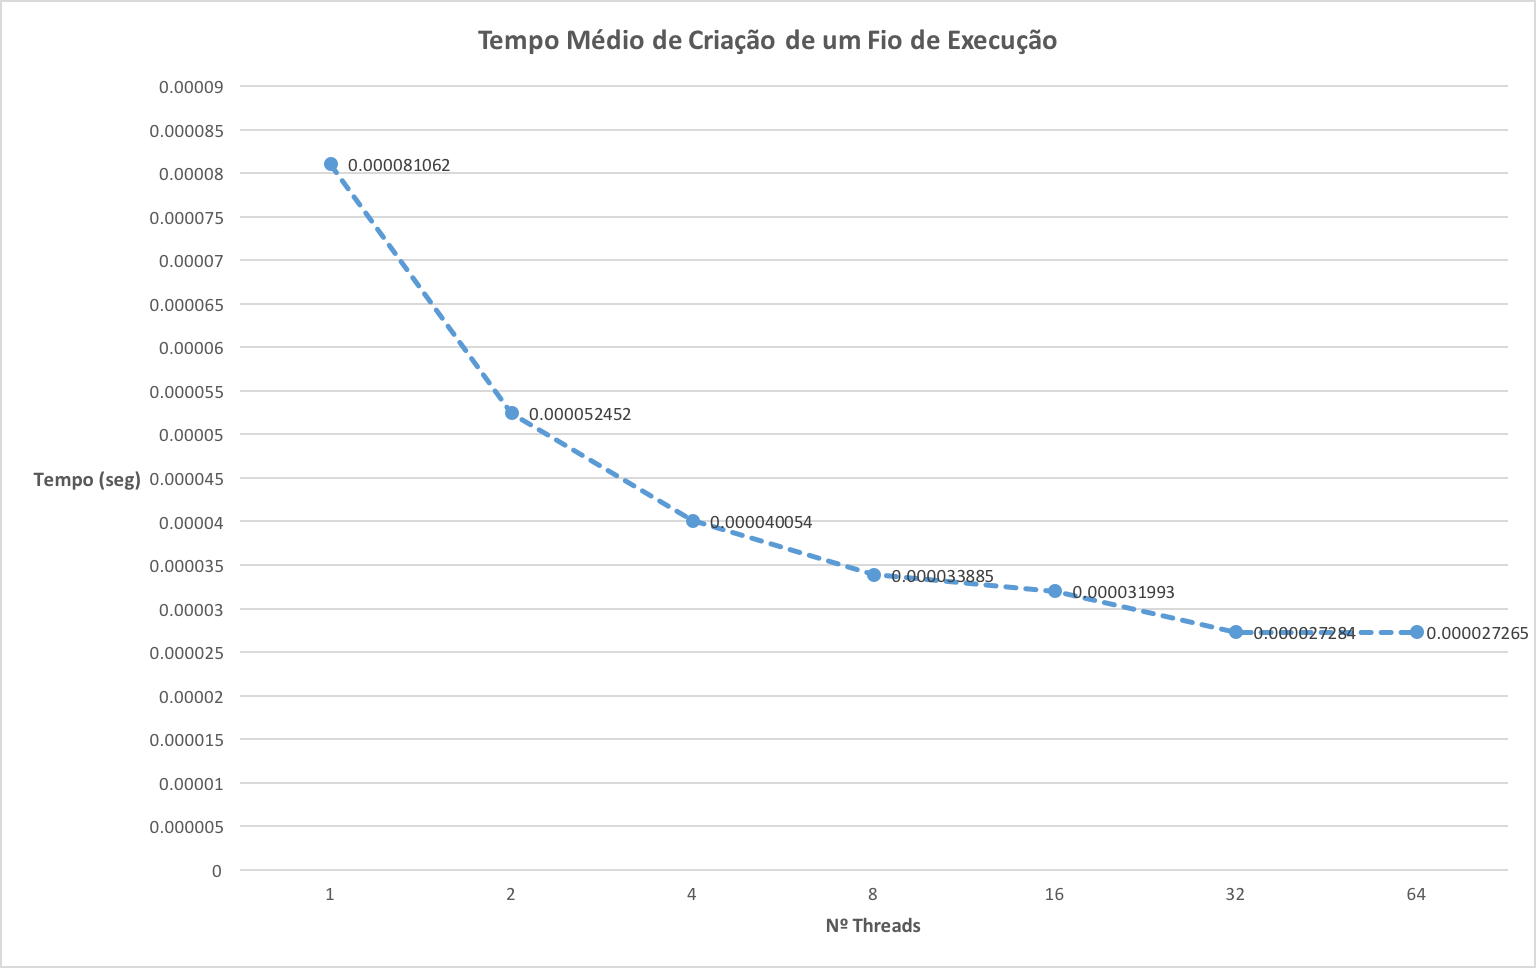
\includegraphics[scale=0.325]{tempo_medio_my_laptop.png}
\caption{Tempo Médio da Criação de um Fio de Execução}
\label{fig:tempo_medio_my_laptop}
\end{figure}

No gráfico da figura \ref{fig:tempo_medio_my_laptop} podemos encontra os resultados obtidos na minha máquina. Como podemos ver pela figura, o tempo médio, quando se cria uma única \textit{Thread} é de 0.000081062 segundos, à medida que vamos aumentando o número de \textit{Threads} o tempo médio vai diminuindo, atingindo 0.000027265 segundos com 64 \textit{Threads}, sendo portanto, um ganho de aproximadamente 3. 

Relativamente aos resultados do \textit{Search}, o gráfico da figura \ref {fig:tempo_medio_search} ilustra os resultados obtidos. A semalhança do que acontece na minha máquina pessoal, os tempos médios diminuem à medida que se aumenta o número de \textit{Threads}, sendo que com 16 \textit{Threads} é quando é atingido o menor tempo médio, subindo ligeiramente a partir dai até às 64 \textit{Threads}.

\begin{figure}[h!]
\centering
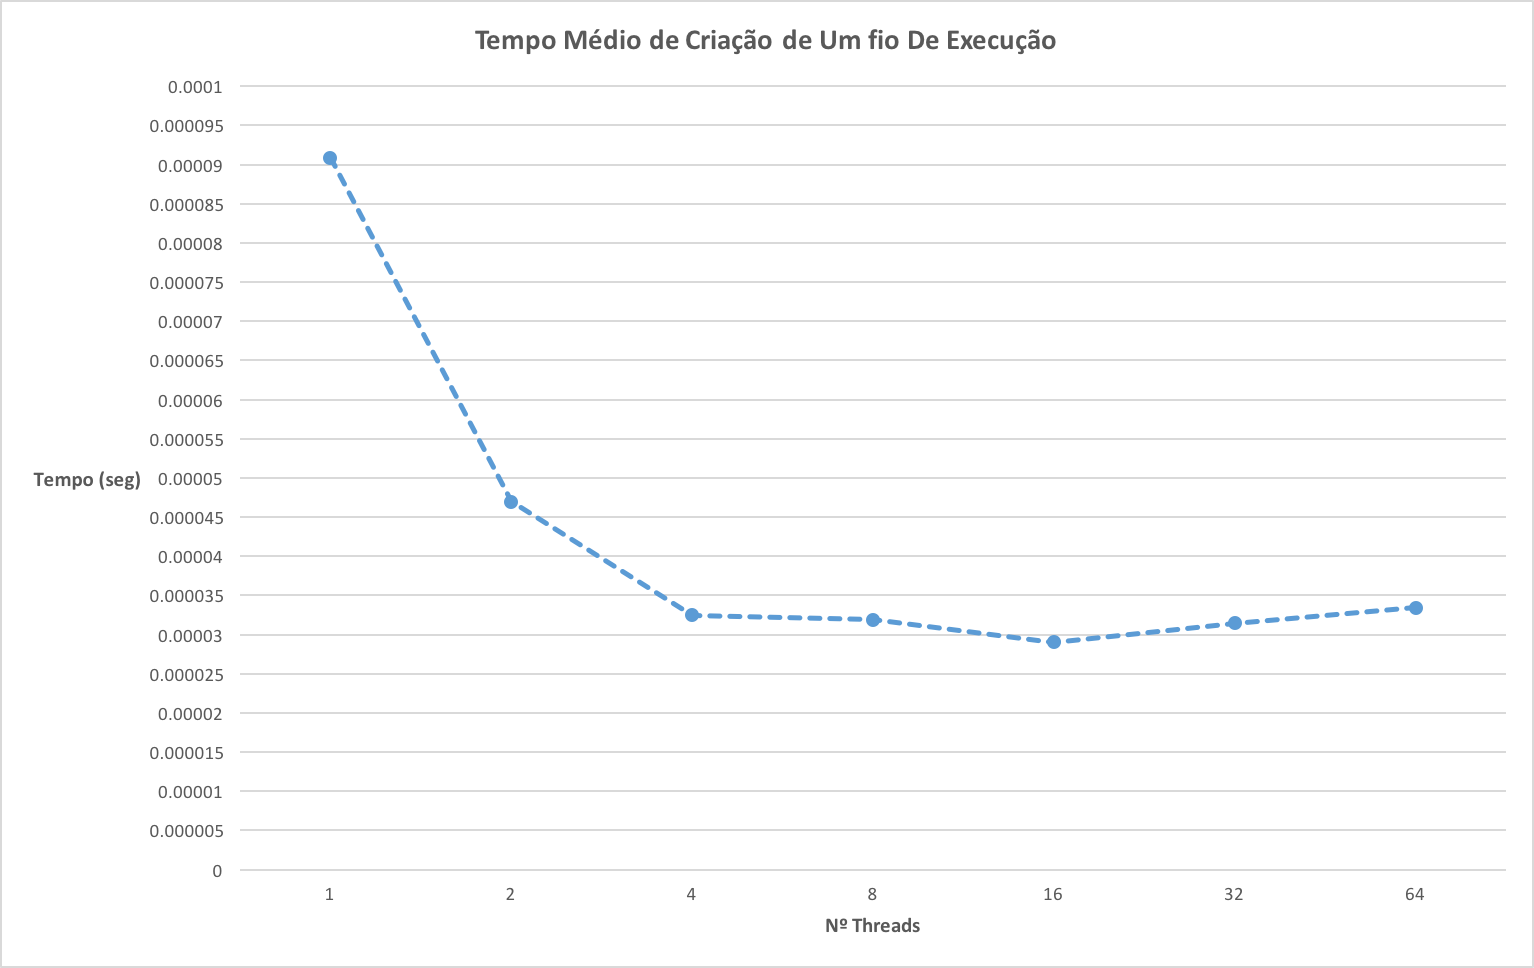
\includegraphics[scale=0.325]{tempo_medio_search.png}
\caption{Tempo Médio da Criação de um Fio de Execução}
\label{fig:tempo_medio_search}
\end{figure}

Em resposta as perguntas efectuadas pelo professor no enunciado, posso dizer que o número de fios de execução (\textit{Threads}) criados, afeta o tempo médio, como podemos constatar pela figura, quanto mais se aumenta o número de \textit{Threads} menor é o tempo médio para a criação de uma \textit{Thread}.

\section{2ª Parte - Regra Trapezoidal\cite{trap_rule}}
\subsection{Caso de Estudo}

A \textbf{Regra Trapezoidal} é uma integração numérica, cujo principal objetivo é aproximar o valor de um integral definido, de uma função, em que não é necessário usar a expressão analítica para a primitiva da função.

Este método usa três fases:
\begin{enumerate}
\item Decompõe-se o domínio em sub-intervalos;
\item Calcula-se uma integração aproximada para cada sub-intervalo;
\item Soma de todos os resultados obtidos.
\end{enumerate}

Este método é usado, porque nem todas as funções tem uma primitiva de forma explícita, é difícil avaliar a primitiva de uma função e sobretudo quando não é possível ter uma expressão analitica para o integral, mas conhece-se os seus valores num conjunto de valores de um intervalo.

A formula matemática para a Regra Trapezoidal é dada por:
\begin{gather*}
\int_{a}^{b} f(x) dx \simeq (b-a) \frac{f(a)+f(b)}{2}
\end{gather*}

Para se perceber melhor a Regra Trapezoidal, suponhamos que temos:
\begin{gather*}
x = a\\
x = b\\
\end{gather*}
e 
\begin{gather*}
x_{n+1} = x_{n} + h  
\end{gather*}
em que
\begin{gather*}
h = \frac{(b-a)}{n}
\end{gather*}
em que \textit{n} é número de sub-intervalos então a Regra Trapezoidal composta é:
\begin{gather*}
\int_{a}^{b}f(x)dx\simeq \frac{h}{2}\left [ f(x_{1})+2f(x_{2})+2f(x_{3})+\cdots +f(x_{n}) \right ]
\end{gather*}

\subsection{Análise dos Resultados}
O algoritmo usa \textit{PThreads}. Depois de criadas \textit{x Threads}, cada \textit{Thread} calcula uma aproximação para um sub-intervalo e no fim soma aos outros resultados das outras \textit{Threads}, de referir que é nessa operação que a variável é partilhada pelas \textit{Threads} (região crítica). Na região critica apliquei as diferentes formas de forçar a exclusão mutua que estudamos (Busy Waiting, mutex e semáforos) de maneira a evitarmos \textit{Data Races}.  
Depois de desenvolvido o algoritmo, procedi a realização de vários testes, como referi em cima foram feitos 5 execuções para cada número de \textit{Threads} (1, 2, 4, 8 ,16, 32 e 64) e extrai o melhor tempo dessas medições. Os meus valores de entrada foram: a=0, b=1024, sendo que n varia, correspondendo ao número de \textit{Threads}. 

O resultado do algoritmo para estes valores é de 357914112. Os resultados obtidos na minha máquina podem ser consultados no gráfico da figura \ref {fig:tempo_varios_kernels_my_laptop}.

\begin{figure}[h!]
\centering
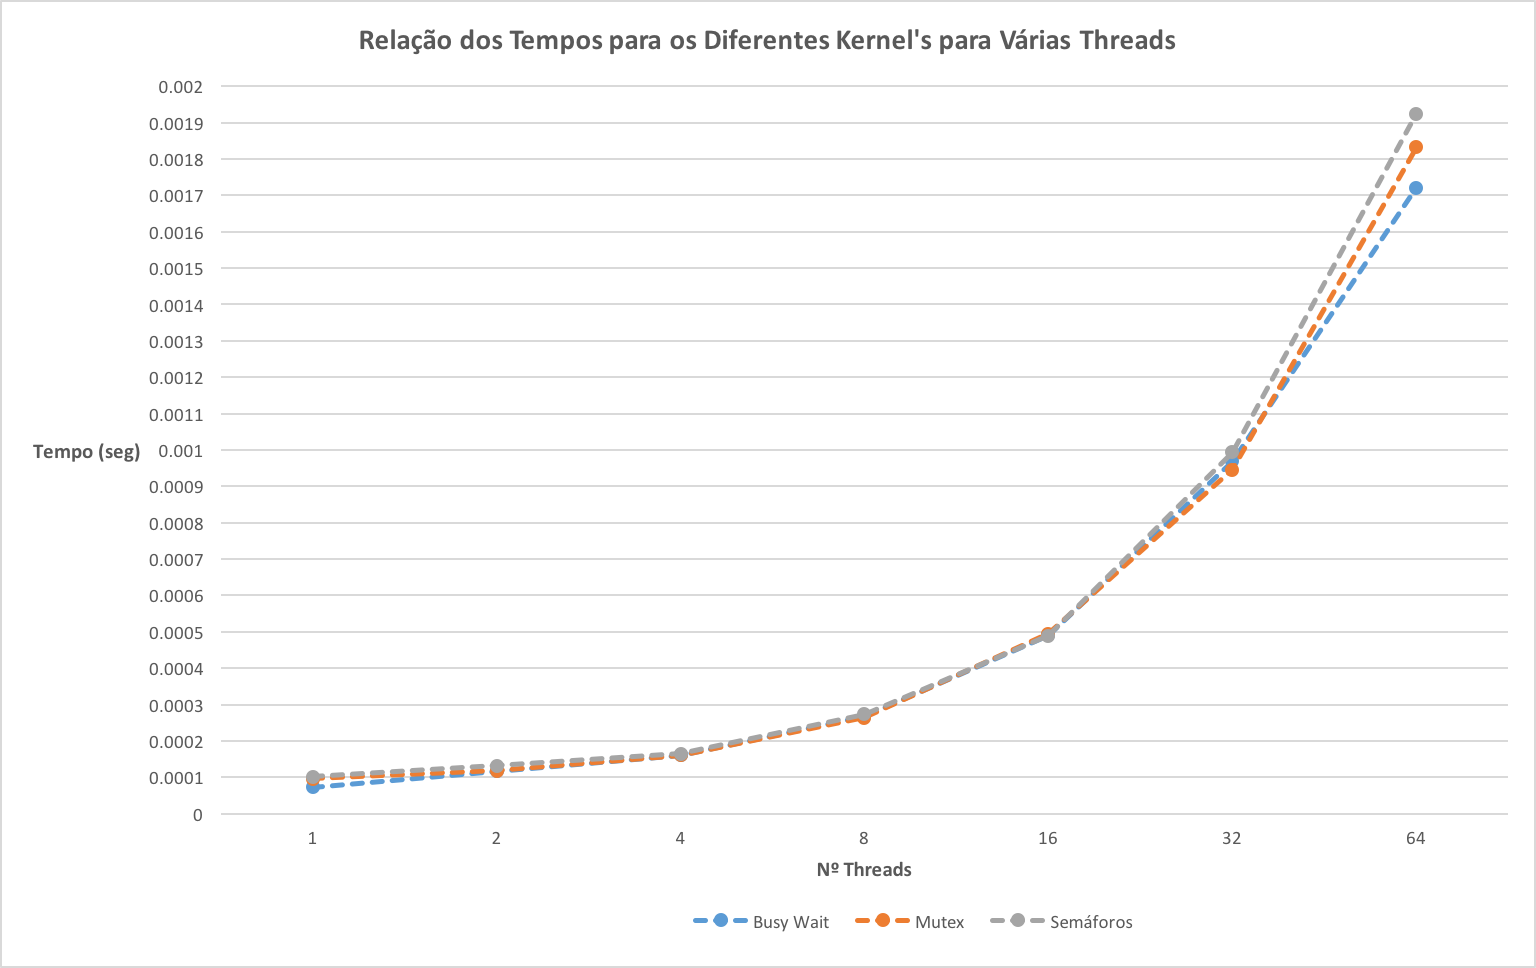
\includegraphics[scale=0.325]{tempos_varios_kernels_my_laptop.png}
\caption{Relação dos Tempos para os Diferentes \textit{Kernel's} para Várias \textit{Threads}}
\label{fig:tempo_varios_kernels_my_laptop}
\end{figure}

Ao analisarmos o gráfico da figura \ref{fig:tempo_varios_kernels_my_laptop}, podemos constatar que o comportamento dos métodos de exclusão mutua, à medida que se aumenta o número de \textit{Threads} é praticamente semelhante para os 3. De referir que com um número de \textit{Threads} de 64 o \textit{Busy Waiting} é o mais eficiente seguido do \textit{Mutex} e por fim dos Semáforos. Com os resultados que obtive na minha máquina não posso concluir que haja um método que seja melhor que os outros todos, uma vez que há alguma variação, por exemplo, com 32 \textit{Threads} o método \textit{Mutex} é melhor que os outros mas com 64 \textit{Threads} já é o método \textit{Busy Waiting} e com 16 \textit{Threads} já é o método dos semáforos (apesar da diferença ser mesmo muito reduzida em relação aos outros).

\begin{figure}[h!]
\centering
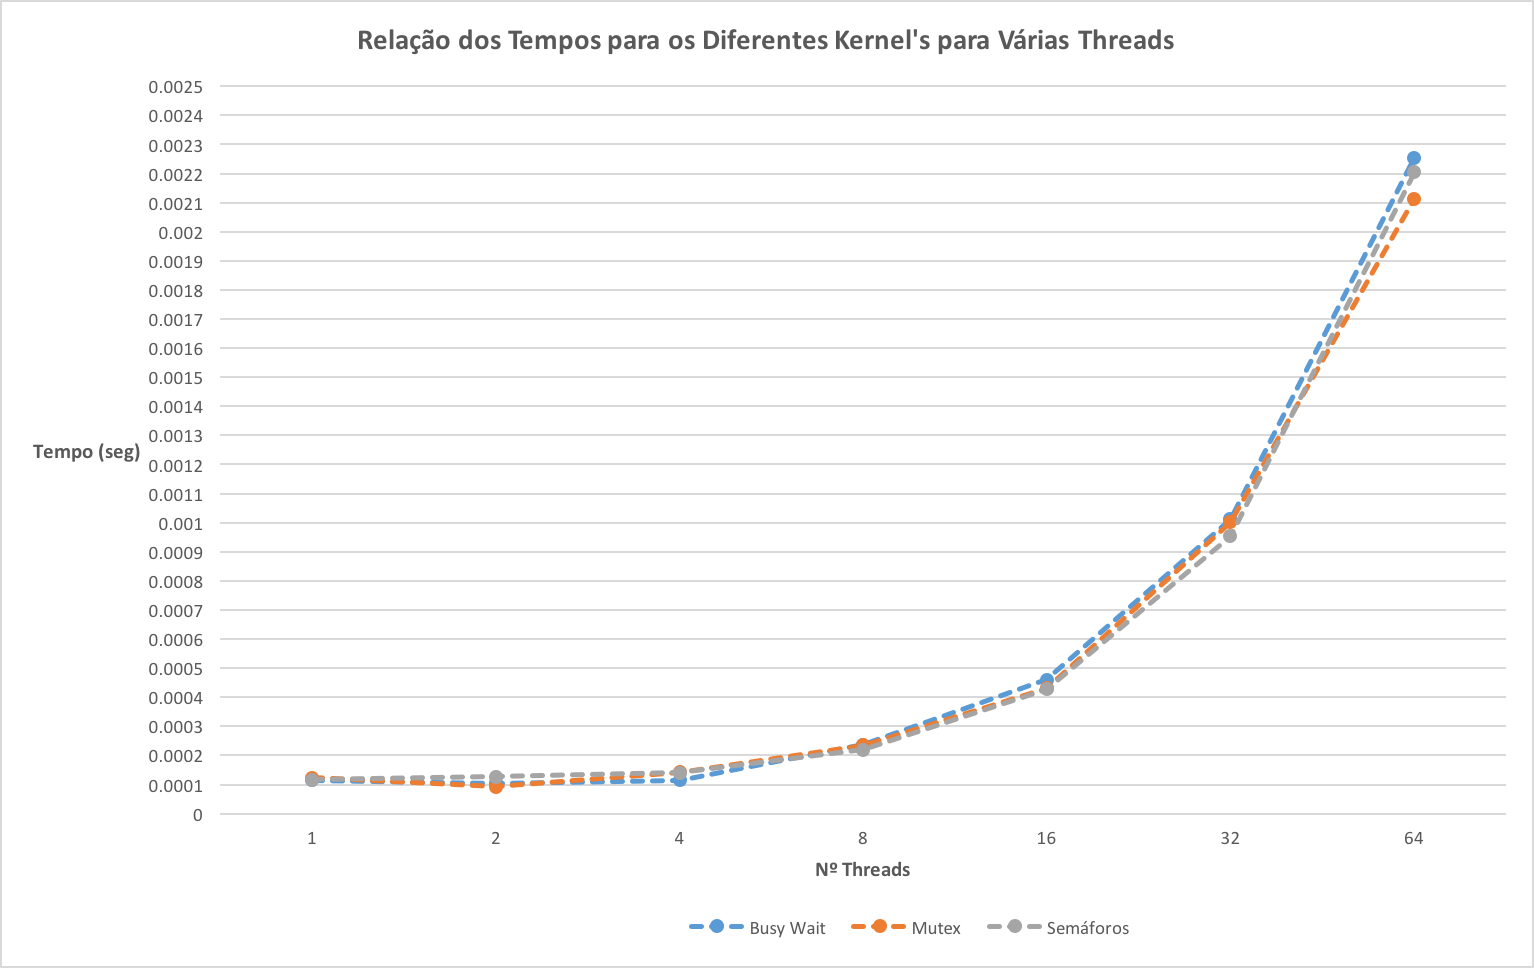
\includegraphics[scale=0.325]{tempos_varios_kernels_search.png}
\caption{Relação dos Tempos para os Diferentes \textit{Kernel's} para Várias \textit{Threads}}
\label{fig:tempo_varios_kernels_search}
\end{figure}

Os resultados obtidos na máquina 431 do \textit{Search} estão ilustrados no gráfico da figura \ref{fig:tempo_varios_kernels_search}. Ao analisarmos o gráfico, podemos constatar que o comportamento dos diferentes \textit{Kernel's} é semelhante ao comportamento destes quando executados na minha máquina, ou seja, á medida que se aumenta o número de \textit{Threads} o tempo de execução dos \textit{Kernel's} também tende a aumentar. Mais uma vez, e também à semelhança do que aconteceu na minha máquina, com estes resultados não podemos concluir que um \textit{Kernel} é melhor que o outro, pois o comportamento dos 3 é muito semelhante. Por exemplo o \textit{Kernel Busy Waiting} é melhor com 4 \textit{Threads}, já o \textit{Kernel} Semáforos é o melhor com 16 e 32 \textit{Threads} e por fim o \textit{Kernel Mutex} é o melhor com 64 \textit{Threads}, posto isto não posso afirmar com certeza qual é o melhor método para forçar a exclusão mutua. 

\subsection{Busy Waitinging}

\begin{itemize}
\item \textbf{Vantagens}
\begin{itemize}
\item Os algortítmos de \textit{Busy Waiting} são fáceis de implementar em qualquer máquina.
\end{itemize}
\item \textbf{Desvantagens}
\begin{itemize}
\item Estes algoritmos são da inteira responsabilidade do programador;
\item Como existem vários processos á espera, a ocupação do \textit{CPU} acaba por ser um desperdício de recursos. Estes processos poderiam ser bloqueados.
\end{itemize}
\end{itemize}

\subsection{Semáforos}
\begin{itemize}
\item \textbf{Vantagens}
\begin{itemize}
\item Em \textit{POSIX} os semáforos podem sincronizar processos com ou sem memória partilhada.
\end{itemize}
\item \textbf{Desvantagens}
\begin{itemize}
\item Uma má programação pode levar a resultados inesperados;
\item Obriga o programador a inserir explicitamente instruções \textit{sem\_wait} ou \textit{sem\_post}.
\end{itemize}
\end{itemize}

\subsection{Mutexes}
\begin{itemize}
\item \textbf{Vantagens}
\begin{itemize}
\item Versão simplificada de um semáforo (não precisa de contar);
\item Só necessita de 1 bit para representar a variáverl mutex (livre,ocupado);
\item São eficientes e fáceis de implementar;
\item Se bem implementados as hipóteses de haver erros é quase 0;
\item Há um melhor aproveitamento do processador.
\end{itemize}
\item \textbf{Desvantagens}
\begin{itemize}
\item São adequados apenas para organizar a exclusão mútua de algum recurso ou parte de código partilhada
\end{itemize}
\end{itemize}

\section{Conclusão}
As \textit{PThreads} ou \textit{POSIX Threads}, como já foi dito em cima, são muito utilizadas em ambientes \textit{Unix}, para criação de \textit{Threads}, com estas podemos facilmente paralelizar o código, de forma a tirar o melhor partido dos recursos que temos disponíveis. Como vimos nas análises dos resultados obtidos para a primeira parte deste trabalho quanto mais \textit{Threads} criámos, menor é o seu tempo de criação.

Para se paralelizar um código usando \textit{PThreads}, é necessário ter em atenção as regiões críticas, estas não podem ser acedidas por mais que uma \textit{Thread} ao mesmo tempo, para isso é necessário implementar mecanismos de exclusão mútua (\textit{Busy Waiting, Mutex} e Semaforos). Estes 3 mecanismos, como vimos, foram implementados e testados em duas máquinas, a minha máquina pessoal e a máquina 431 do \textit{Search}, das quais obtive os resultados em cima apresentados, resultados esses que não me permitem concluir qual é o mecanismo/método mais eficiente para implementar exclusão mutua. 

Apesar de não ter obtido dados muito esclarecedores, penso que a implementação de exclusão mutua será mais eficiente/segura se usarmos semáforos ou \textit{Mutex}, embora o \textit{Mutex} seja apenas adequado para uma parte de código ou algum recurso partilhado. Penso que estes dois métodos são os mais eficientes/seguros pois são os que tem menor margem de erro e como tal a ocorrência de \textit{Data Races} é pouco provável, para além disso, permite-nos tirar um maior partido dos recursos que dispomos.

Na realização deste trabalho não me deparei com grandes dificuldades, uma vez que era um trabalho simples, e curto. Contudo confesso que não estou satisfeito com os meus resultados, isto porque, não era bem estes resultados que estava à espera. Esperava que os tempos de execução dos 3 \textit{Kernel's} fossem mais esclarecedores do que aqueles que obtive, posto isto como trabalho futuro pretendo debruçar-me melhor sobre o algoritmo, apesar de achar que este está bem implementado, mas gostava de perceber o porquê de estes resultados não terem sido os que esperava. Quanto ao restante trabalho faço um balanço bastante positivo.






% An example of a floating figure using the graphicx package.
% Note that \label must occur AFTER (or within) \caption.
% For figures, \caption should occur after the \includegraphics.
% Note that IEEEtran v1.7 and later has special internal code that
% is designed to preserve the operation of \label within \caption
% even when the captionsoff option is in effect. However, because
% of issues like this, it may be the safest practice to put all your
% \label just after \caption rather than within \caption{}.
%
% Reminder: the "draftcls" or "draftclsnofoot", not "draft", class
% option should be used if it is desired that the figures are to be
% displayed while in draft mode.
%
%\begin{figure}[!t]
%\centering
%\includegraphics[width=2.5in]{myfigure}
% where an .eps filename suffix will be assumed under latex, 
% and a .pdf suffix will be assumed for pdflatex; or what has been declared
% via \DeclareGraphicsExtensions.
%\caption{Simulation results for the network.}
%\label{fig_sim}
%\end{figure}

% Note that the IEEE typically puts floats only at the top, even when this
% results in a large percentage of a column being occupied by floats.


% An example of a double column floating figure using two subfigures.
% (The subfig.sty package must be loaded for this to work.)
% The subfigure \label commands are set within each subfloat command,
% and the \label for the overall figure must come after \caption.
% \hfil is used as a separator to get equal spacing.
% Watch out that the combined width of all the subfigures on a 
% line do not exceed the text width or a line break will occur.
%
%\begin{figure*}[!t]
%\centering
%\subfloat[Case I]{\includegraphics[width=2.5in]{box}%
%\label{fig_first_case}}
%\hfil
%\subfloat[Case II]{\includegraphics[width=2.5in]{box}%
%\label{fig_second_case}}
%\caption{Simulation results for the network.}
%\label{fig_sim}
%\end{figure*}
%
% Note that often IEEE papers with subfigures do not employ subfigure
% captions (using the optional argument to \subfloat[]), but instead will
% reference/describe all of them (a), (b), etc., within the main caption.
% Be aware that for subfig.sty to generate the (a), (b), etc., subfigure
% labels, the optional argument to \subfloat must be present. If a
% subcaption is not desired, just leave its contents blank,
% e.g., \subfloat[].


% An example of a floating table. Note that, for IEEE style tables, the
% \caption command should come BEFORE the table and, given that table
% captions serve much like titles, are usually capitalized except for words
% such as a, an, and, as, at, but, by, for, in, nor, of, on, or, the, to
% and up, which are usually not capitalized unless they are the first or
% last word of the caption. Table text will default to \footnotesize as
% the IEEE normally uses this smaller font for tables.
% The \label must come after \caption as always.
%
%\begin{table}[!t]
%% increase table row spacing, adjust to taste
%\renewcommand{\arraystretch}{1.3}
% if using array.sty, it might be a good idea to tweak the value of
% \extrarowheight as needed to properly center the text within the cells
%\caption{An Example of a Table}
%\label{table_example}
%\centering
%% Some packages, such as MDW tools, offer better commands for making tables
%% than the plain LaTeX2e tabular which is used here.
%\begin{tabular}{|c||c|}
%\hline
%One & Two\\
%\hline
%Three & Four\\
%\hline
%\end{tabular}
%\end{table}


% Note that the IEEE does not put floats in the very first column
% - or typically anywhere on the first page for that matter. Also,
% in-text middle ("here") positioning is typically not used, but it
% is allowed and encouraged for Computer Society conferences (but
% not Computer Society journals). Most IEEE journals/conferences use
% top floats exclusively. 
% Note that, LaTeX2e, unlike IEEE journals/conferences, places
% footnotes above bottom floats. This can be corrected via the
% \fnbelowfloat command of the stfloats package.




% trigger a \newpage just before the given reference
% number - used to balance the columns on the last page
% adjust value as needed - may need to be readjusted if
% the document is modified later
%\IEEEtriggeratref{8}
% The "triggered" command can be changed if desired:
%\IEEEtriggercmd{\enlargethispage{-5in}}

% references section

% can use a bibliography generated by BibTeX as a .bbl file
% BibTeX documentation can be easily obtained at:
% http://mirror.ctan.org/biblio/bibtex/contrib/doc/
% The IEEEtran BibTeX style support page is at:
% http://www.michaelshell.org/tex/ieeetran/bibtex/
%\bibliographystyle{IEEEtran}
% argument is your BibTeX string definitions and bibliography database(s)
%\bibliography{IEEEabrv,../bib/paper}
%
% <OR> manually copy in the resultant .bbl file
% set second argument of \begin to the number of references
% (used to reserve space for the reference number labels box)

\bibliographystyle{abbrv}
\bibliography{ref.bib}


% that's all folks
\end{document}


